A representação da arquitetura para este projeto pode ser visualizada por meio do um diagrama apresentado na Figura \ref{img:diagrama_arquitetura}.

\begin{figure}[H]
	\centering
	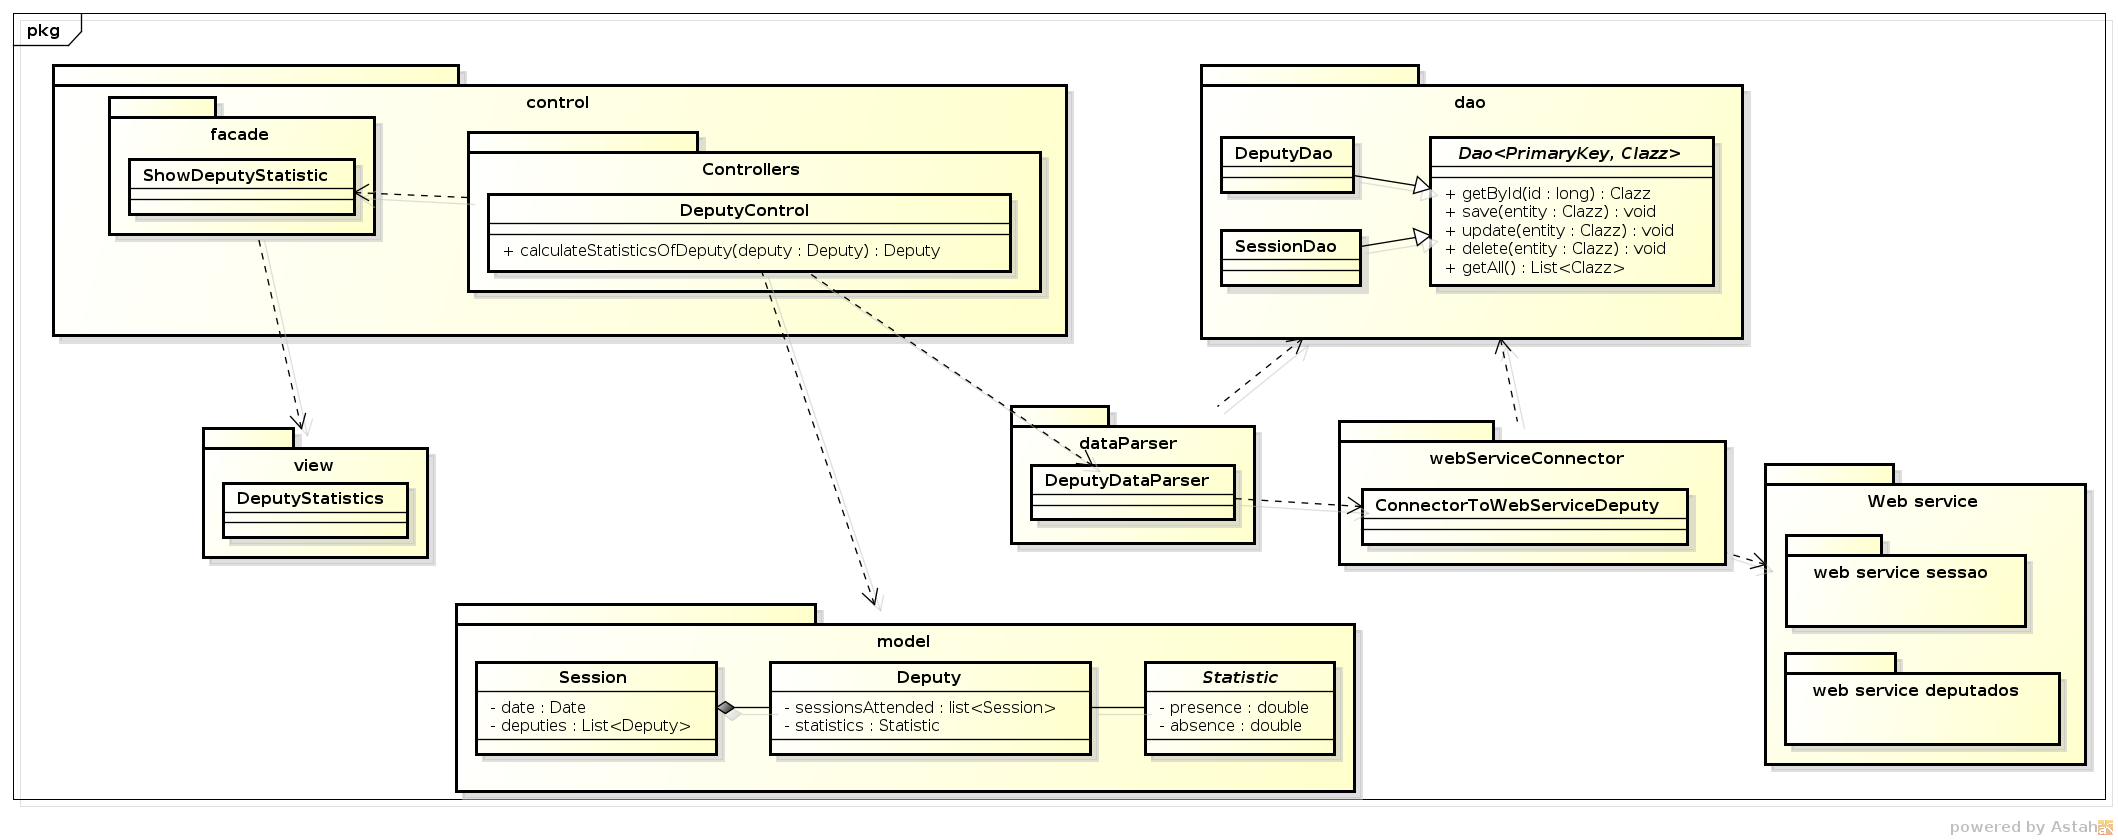
\includegraphics[width=1\textwidth]{arquitetura/arquitetura_sprint1}
	\caption{Diagrama da arquitetura do sistema}
	\label{img:diagrama_arquitetura}
\end{figure}

A arquitetura do \textit{Chamada Parlamentar} foi projetada com o objetivo de tornar o \textit{software} leve e eficiente. A confiança nos dados apresentados pelo sistema se dá pela utilização de duas formas de obtenção dos dados em momento de execução. A primeira forma, e mais atualizada, ou seja, mais confiável, é a disponibilização dos dados via \textit{WebService}.

Caso haja algum problema na conexão com o \textit{WebService}, o sistema fará a obtenção dos dados via Banco de Dados, onde estão armazenados os dados do \textit{WebService} do dia anterior. O sistema fará a atualização do banco de dados todos os dias as 5 horas da manhã.

O pacote \textit{WebServiceConnector} será utilizado para realizar a conexão com o \textit{WebService} e o \textit{dataParser} irá tratar os dados da forma apropriada para armazenamento dos mesmos no banco ou disponibilização dos mesmos, ou seja, estes dois pacotes sempre irão trabalhar lado a lado.

O \textit{Dao} será o pacote que fará a conexão e todas as manupulações necessárias no Banco de Dados. Tanto para edição de dados quanto para obtenção dos mesmos no Banco de Dados.

Os pacotes utilizados para a manipulação dos dados em nivel de Base de Dados são o grande diferencial desta arquitetura. O restante é o que forma o conhecido \textit{MVC}, a \textit{modelo}, a \textit{view} e a \textit{controler}.